\documentclass[10pt,a4paper]{article}
\usepackage{amsmath,amssymb,amsfonts}
\usepackage{graphicx}
\usepackage[margin=0.85in]{geometry}
\usepackage{hyperref}
\usepackage{titling}
\usepackage{titlesec}
\usepackage{mathpazo}
\usepackage{microtype}
\usepackage{parskip}
\usepackage{enumitem}
\usepackage{booktabs}
\usepackage{multirow}
\usepackage{caption}
\usepackage{float}
\usepackage{tikz}
\usetikzlibrary{trees,shapes,shapes.geometric,arrows.meta,positioning,calc}

\setlist{nosep}

\newcommand{\E}{\mathbb{E}}
\newcommand{\Var}{\mathrm{Var}}
\newcommand{\Prob}{\mathbb{P}}

\hypersetup{colorlinks=true,linkcolor=blue,citecolor=blue,urlcolor=blue}

% %control spacing
% \titlespacing*{\section}{0pt}{0.6em}{4pt}
% \titlespacing*{\subsection}{0pt}{0.4em}{3pt}
% \titlespacing*{\subsubsection}{0pt}{0.3em}{2pt}

%bring title up
\setlength{\droptitle}{-5em}

\title{3E3 Modelling Risk Coursework \\ \large \textit{Integrated Risk Analysis for GreenCo Energy}}
\author{Liu Zihe -- zl559}
\date{University of Cambridge -- 10 March 2026}

\begin{document}

\maketitle

%========================================================================================
\section{Introduction}
%========================================================================================

GreenCo Energy is developing a coastal renewable energy hub integrating offshore wind generation, on-site hydrogen production via electrolysis, and a heavy goods vehicle (HGV) refuelling station. The project faces four interlinked sources of uncertainty: \textbf{demand volatility} (stochastic monthly hydrogen demand), \textbf{production variability} (electrolyser availability), \textbf{congestion risk} (queueing at the refuelling station), and \textbf{long-term investment uncertainty} (demand growth trajectory and competitor entry).

This report develops an integrated risk analysis. Four models are applied, each addressing a different risk source: (1)~\textit{Newsvendor model} for the monthly production decision under demand uncertainty; (2)~\textit{M/M/$s$ queueing model} for refuelling station congestion; (3)~\textit{Decision tree} for multi-stage strategy evaluation under scenario uncertainty; (4)~\textit{Monte Carlo simulation} for full NPV distributions and downside risk measurement. The objective is to maximise expected NPV while explicitly assessing downside risk exposure and service-level compliance.

%========================================================================================
\section{Problem Setup}
\label{sec:setup}
%========================================================================================

\subsection{Analytical Models}

We use the newsvendor inventory production model for computing the expected profit $\E[\Pi_t]$ and optimal production quantity at year $t$, $Q_t^*$. We also use a M/M/s queueing model to model refuelling service. Our parameters for these models, and demand growth models, are shown in Table \ref{tab:params}. Exact details are explained in section \ref{sec:analysis}.

\begin{table}[H]
    \centering
    \caption{Model parameters.}
    \label{tab:params}
    \footnotesize
    \begin{tabular}{@{}lll@{}}
        \toprule
        \textbf{Symbol}    & \textbf{Parameter}                                & \textbf{Value}               \\
        \midrule
        \multicolumn{3}{@{}l}{\textit{Demand \& Pricing}}                                                     \\
        $\mu_0$            & Initial mean monthly demand                       & 1000 t                       \\
        $\sigma_0$         & Initial demand std.\ deviation                    & 150 t                        \\
        $\mathrm{CV}$      & Coefficient of variation ($\sigma_t/\mu_t$)       & 0.15                         \\
        $\mu_t$            & Year-$t$ mean monthly demand                      & Eqn~\eqref{eq:demand_growth} \\
        $\sigma_t$         & Year-$t$ standard deviation of monthly demand     & Eqn~\eqref{eq:demand_growth} \\
        $p$                & Selling price                                     & \pounds4000/t                \\
        $c_p$              & Production cost                                   & \pounds2500/t                \\
        $c_s$              & Spot market purchase price                        & \pounds3200/t                \\
        $c_h$              & Storage/handling cost (unsold)                    & \pounds300/t                 \\
        \midrule
        \multicolumn{3}{@{}l}{\textit{Production Capacity}}                                                   \\
        $K_{\mathrm{nom}}$ & Nominal electrolyser capacity                     & 40 t/day                     \\
        $\alpha$           & Operational availability                          & 85\%                         \\
        $n_d$              & Days per month                                    & 30                           \\
        \midrule
        \multicolumn{3}{@{}l}{\textit{Refuelling Station}}                                                    \\
        $\lambda$          & HGV arrival rate                                  & 10 vehicles/hr               \\
        $1/\mu$            & Mean refuelling time                              & 12 min                       \\
        $s_0$              & Initial number of bays                            & 3                            \\
        $W_q^{\max}$       & Maximum average queue wait                        & 5 min                        \\
        \midrule
        \multicolumn{3}{@{}l}{\textit{Growth \& Discounting}}                                                 \\
        $p_H$              & Probability of high growth                        & 0.45                         \\
        $g_H,\,g_L$        & Annual growth rates (mean demand)                 & 10\%, 3\%                    \\
        $p_C$              & Probability of competitor entry (high growth, Y3) & 0.40                         \\
        $\delta$           & Demand reduction from competitor                  & 15\%                         \\
        $r$                & Discount rate                                     & 7\%/yr                       \\
        \bottomrule
    \end{tabular}
\end{table}

\subsection{Demand Growth and Scenarios}

Monthly hydrogen demand in year $t$: $D_t \sim \mathcal{N}(\mu_t, \sigma_t^2)$, with constant $\mathrm{CV} = \sigma_t/\mu_t = 0.15$, and annual growth rate of mean demand $g$ ($g_H=0.1$ for high growth, and $g_L=0.03$ for low growth) gives:
\begin{equation}
    \mu_t = \mu_0(1+g)^t, \qquad \sigma_t = \mathrm{CV}\cdot\mu_t
    \label{eq:demand_growth}
\end{equation}
With competitor entry (high growth scenario, $t \geq 3$): $\mu_t^{\mathrm{comp}} = (1-\delta)\mu_t$. This gives three terminal scenarios:

\begin{table}[H]
    \centering
    \caption{Scenario probabilities and monthly demand ($\mu_t$ in t/month, $\sigma_t$ in t/month).}
    \label{tab:demand}
    \small
    \begin{tabular}{@{}lcccccc@{}}
        \toprule
        \textbf{Scenario}        & \multicolumn{2}{c}{\textbf{High, no comp.}} & \multicolumn{2}{c}{\textbf{High + comp.}} & \multicolumn{2}{c}{\textbf{Low growth}}                                     \\
        $\Prob(\text{scenario})$ & \multicolumn{2}{c}{$p_H(1-p_C) = 0.27$}     & \multicolumn{2}{c}{$p_H p_C = 0.18$}      & \multicolumn{2}{c}{$1-p_H = 0.55$}                                          \\
        \cmidrule(lr){2-3}\cmidrule(lr){4-5}\cmidrule(lr){6-7}
        \textbf{Yr}              & $\mu_t$                                     & $\sigma_t$                                & $\mu_t$                                 & $\sigma_t$ & $\mu_t$ & $\sigma_t$ \\
        \midrule
        0                        & 1000                                        & 150                                       & 1000                                    & 150        & 1000    & 150        \\
        1                        & 1100                                        & 165                                       & 1100                                    & 165        & 1030    & 155        \\
        2                        & 1210                                        & 182                                       & 1210                                    & 182        & 1061    & 159        \\
        3                        & 1331                                        & 200                                       & 1131                                    & 170        & 1093    & 164        \\
        4                        & 1464                                        & 220                                       & 1245                                    & 187        & 1126    & 169        \\
        \bottomrule
    \end{tabular}
\end{table}

\subsection{Investment Strategies}
\label{sec:strategies}

GreenCo must choose one of three strategies at Year~0 to scale its hydrogen infrastructure over a 4-year horizon. Each strategy modifies a different subset of the newsvendor parameters $(c_s, \sigma_t, \bar{Q})$ and the queueing parameter $s$, creating distinct risk--return profiles.

\textbf{Strategy~1 (Immediate Scale-Up).} Invest \pounds54M upfront (\pounds48M electrolyser expansion + \pounds6M for two additional refuelling bays) to increase capacity from $K_\mathrm{nom} = 40$ to 65~t/day at 95\% availability, giving $\bar{Q}_{S1} = 1852.5$~t/mo, and $s = 5$ bays. No changes to demand uncertainty or spot pricing. The bet is that high capacity eliminates spot procurement: since $\bar{Q}_{S1} \gg \mu_t$ for all $t$, the capacity constraint in the newsvendor never binds. However, the risk is overcapacity under the low growth scenario --- demand utilisation $\mu_t/\bar{Q}_{S1}$ falls below 65\% from Y2, triggering a \pounds150/t scale-inefficiency penalty that inflates $c_p$ to \pounds2650/t.

\textbf{Strategy~2 (Flexibility and Risk Mitigation).} Invest \pounds20M upfront in modular storage, demand-smoothing contracts, and digital forecasting. This does not expand capacity ($\bar{Q}$, $s$ are unaffected), but instead reduces two key newsvendor cost drivers: demand volatility drops by 40\% ($\sigma_t \to 0.6\sigma_t = 0.09\mu_t$), and pre-negotiated contingent contracts lower spot procurement cost to $c_s = \text{\pounds}2900$/t. The reduced $c_s$ shifts the critical ratio from $F(Q^*) = 0.200$ to $F(Q^*) = 0.125$, pushing the optimal production quantity further below the mean; simultaneously, the tighter demand distribution ($\sigma \downarrow$) reduces both $\mathrm{ELS}$ and $\mathrm{ELOI}$, cutting procurement and storage waste. Under high growth, capacity eventually binds ($Q_t^* > \bar{Q}$ from Y3), forcing systematic spot reliance.

\textbf{Strategy~3 (Staged Expansion).} Invest \pounds8M upfront in expandable foundations and grid upgrades, preserving the option to scale later. This is a \textit{real-options} structure: at the end of Y1, after observing demand growth, GreenCo chooses one of two branches:
\begin{itemize}
    \item \textit{High growth observed} $\to$ expand nominal capacity $K_\mathrm{nom} = $ 65~t/day at $\alpha=95\%$ availability for \pounds42M (discounted by the pre-installed foundations), matching S1 specifications from Y2 onward.
    \item \textit{Low growth observed} $\to$ invest \pounds15M in flexibility measures (a reduced version of S2: same $\sigma$ reduction and $c_s = \text{\pounds}2900$/t), matching S2 specifications from Y2 onward.
\end{itemize}
The cost of deferral is a 10\% realised revenue reduction in Y1--Y2 under both growth paths. Until the Y1 decision, capacity and parameters remain at baseline.

Table~\ref{tab:strategy_params} summarises the parameter modifications. All unmodified parameters retain their base-case values from Table~\ref{tab:params}.

\begin{table}[H]
    \centering
    \caption{Strategy-specific parameter modifications (base: $\bar{Q} = 1020$ t/mo, $s = 3$ bays, $c_s = \text{\pounds}3200$/t, $\sigma_t = 0.15\mu_t$).}
    \label{tab:strategy_params}
    \small
    \begin{tabular}{@{}llll@{}}
        \toprule
        \textbf{Parameter}       & \textbf{Strategy 1}     & \textbf{Strategy 2} & \textbf{Strategy 3}             \\
        \midrule
        $I_0$ (Year 0)           & \pounds54M              & \pounds20M          & \pounds8M                       \\
        $I_1$ (Year 1)           & ---                     & ---                 & \pounds42M (H) / \pounds15M (L) \\
        Capacity $\bar{Q}$       & 1852.5 t/mo             & 1020 t/mo           & 1020 $\to$ 1852.5 (H branch)    \\
        Availability             & 95\%                    & 85\%                & 85\% $\to$ 95\% (H branch)      \\
        Bays $s$                 & 5                       & 3                   & 3                               \\
        $\sigma_t$               & $0.15\mu_t$             & $0.09\mu_t$         & $0.15\mu_t$                     \\
        $c_s$                    & \pounds3200/t           & \pounds2900/t       & \pounds3200/t                   \\
        Revenue                  & 100\%                   & 100\%               & 90\% in Y1--Y2                  \\
        Low-growth $c_p$ penalty & $+$\pounds150/t from Y2 & ---                 & ---                             \\
        \bottomrule
    \end{tabular}
\end{table}

%========================================================================================
\section{Operational Risk Analysis}
\label{sec:analysis}
%========================================================================================

\subsection{Monthly Production Decision: Newsvendor Model}
\label{sec:newsvendor}

Each month GreenCo chooses production quantity $Q \in [0,\bar{Q}]$ before demand $D \sim \mathcal{N}(\mu_t,\sigma_t^2)$ is realised. The effective monthly capacity is:
\begin{equation}
    \bar{Q} = K_{\mathrm{nom}} \cdot \alpha \cdot n_d
    \label{eq:capacity}
\end{equation}
All demand is contractually met; shortfalls are covered by spot procurement. Monthly profit:
\begin{equation}
    \Pi(Q,D) = \underbrace{pD}_{\text{revenue}} - \underbrace{c_p Q}_{\text{production}} - \underbrace{c_s\max(D-Q,0)}_{\text{spot procurement}} - \underbrace{c_h\max(Q-D,0)}_{\text{storage}}
    \label{eq:profit}
\end{equation}
Taking expectations over demand $D$, we define \textit{expected lost sales} (demand unmet by own production) and \textit{expected leftover inventory} (unsold overproduction):
\begin{equation}
    \text{ELS}(Q) = \E_D[\max(D-Q,0)], \qquad \text{ELOI}(Q) = \E_D[\max(Q-D,0)]
\end{equation}
Since revenue $pD$ is independent of $Q$ (contractual obligation), expected monthly profit is:
\begin{equation}
    \E[\Pi(Q)] = p\mu_t - c_p Q - c_s\,\text{ELS}(Q) - c_h\,\text{ELOI}(Q)
    \label{eq:exp_profit}
\end{equation}

\subsubsection{Optimal Production Quantity}

Note $\frac{d}{dQ}\text{ELS} = -(1-F(Q))$ and $\frac{d}{dQ}\text{ELOI} = F(Q)$, where $F$ is the CDF of demand $D$. Setting $d\E[\Pi]/dQ = 0$:
\begin{equation}
    \frac{d\E[\Pi]}{dQ} = -c_p + c_s\bigl(1-F(Q)\bigr) - c_h F(Q) = 0 \quad\Longrightarrow\quad \boxed{F(Q^*) = \frac{c_s - c_p}{c_s + c_h} = \frac{c_u}{c_u+c_o}}
    \label{eq:critical_ratio}
\end{equation}

This is the \textit{newsvendor critical ratio}, where $c_u = c_s - c_p$ is the underage cost (extra cost of spot vs own production) and $c_o = c_p + c_h$ is the overage cost (production + storage on unsold units, with zero salvage). For normal demand $D \sim \mathcal{N}(\mu_t, \sigma_t^2)$, the capacity-constrained optimum at year $t$ is:
\begin{equation}
    Q_t^* = \min\bigl(\mu_t + z^*\sigma_t,\;\bar{Q}\bigr), \qquad z^* = \Phi^{-1}\!\left(\frac{c_u}{c_u+c_o}\right)
    \label{eq:Q_star}
\end{equation}
where $\Phi^{-1}$ is the inverse CDF of the standard normal distribution.

\subsubsection{Expected Profit Components}

For normal demand, the standard normal loss function $L(z) = \phi(z) - z[1-\Phi(z)]$ gives closed-form expressions for ELS and ELOI. Writing $z_t = (Q_t^* - \mu_t)/\sigma_t$:
\begin{align}
    \mathrm{ELS}(Q_t^*)  & = \sigma_t\, L(z_t)                &  & \text{(expected spot procurement volume)} \\
    \mathrm{ELOI}(Q_t^*) & = \sigma_t\bigl[z_t + L(z_t)\bigr] &  & \text{(expected unsold overproduction)}
\end{align}
The expected annual profit for strategy $k$ in scenario $j$ at year $t$ is:
\begin{equation}
    \E[\Pi_t^{(k,j)}] = 12\Bigl(\alpha_t^{(k)}\, p\mu_t^{(j)} - c_p^{(k)}\, Q_t^{*(k,j)} - c_s^{(k)}\,\mathrm{ELS}(Q_t^{*(k,j)}) - c_h\,\mathrm{ELOI}(Q_t^{*(k,j)})\Bigr)
    \label{eq:annual_profit}
\end{equation}
where $\alpha_t^{(k)}$ is the revenue realisation factor ($\alpha = 0.9$ for S3 in Y1--Y2 due to deferral costs; $\alpha = 1$ otherwise), $\mu_t^{(j)}$, $\sigma_t^{(j)}$ come from Table~\ref{tab:demand}, and $c_s^{(k)}$, $c_p^{(k)}$, $\bar{Q}^{(k)}$ are from Table~\ref{tab:strategy_params}.

\subsubsection{Profit Evolution Under Various Demand Growth and Investment Strategies}

When the capacity constraint does not bind, $z_t = z^*$ and $Q_t^*$ scales linearly with $\mu_t$. Once demand growth pushes $\mu_t + z^*\sigma_t > \bar{Q}$, the constraint binds: $Q_t^* = \bar{Q}$, $z_t$ falls below $z^*$, and $\mathrm{ELS}$ grows rapidly as demand outpaces production. Under high growth with base capacity, this occurs from Year~2 onward. This is the principal mechanism forcing emergency spot procurement under Strategies~2 and~3 (before expansion).

Table~\ref{tab:nv_annual} summarises expected annual profit $\E[\Pi_t^{(k,j)}]$ under each strategy $k \in \{S1, S2, S3\}$, scenario $j \in \{\textit{High-Growth+No Competition, High-Growth+Competition, Low-Growth}\}$, and year $t \in \{0,1,2,3,4\}$. We recalculate $\E[\Pi_t^{(k,j)}]$ using Eqn \ref{eq:annual_profit} based on the modelling changes made to our parameters: effective capacity $\bar{Q}$ under strategy $k$, $\sigma_t$, $c_s$ and $c_p$ etc.

\begin{table}[H]
    \centering
    \caption{Expected annual profit $\E[\Pi_t^{(k,j)}]$ (£M) by strategy, scenario, and year.}
    \label{tab:nv_annual}
    \small
    \begin{tabular}{@{}llrrrr@{}}
        \toprule
        \textbf{Strategy} & \textbf{Scenario} & \textbf{Y1} & \textbf{Y2} & \textbf{Y3} & \textbf{Y4} \\
        \midrule
        \multirow{3}{*}{S1}
                          & High, no comp.    & 17.86       & 19.65       & 21.61       & 23.77       \\
                          & High + comp.      & 17.86       & 19.65       & 18.37       & 20.21       \\
                          & Low growth        & 16.72       & 15.58       & 16.05       & 16.53       \\
        \midrule
        \multirow{3}{*}{S2}
                          & High, no comp.    & 19.02       & 20.80       & 22.46       & 24.22       \\
                          & High + comp.      & 19.02       & 20.80       & 19.56       & 21.29       \\
                          & Low growth        & 17.81       & 18.34       & 18.89       & 19.46       \\
        \midrule
        \multirow{3}{*}{S3}
                          & High, no comp.    & 12.58       & 13.84       & 21.61       & 23.77       \\
                          & High + comp.      & 12.58       & 13.84       & 18.37       & 20.21       \\
                          & Low growth        & 11.78       & 13.25       & 18.89       & 19.46       \\
        \bottomrule
    \end{tabular}
\end{table}

Key observations: (i)~S2 consistently produces higher annual profit than S1 in every scenario and year, despite identical revenue---the reduced spot price (\pounds2900/t) and tighter demand distribution (lower $\sigma$) jointly reduce procurement and storage costs; (ii)~S1's low-growth profits fall sharply in Y2--Y4 due to the \pounds150/t scale-inefficiency penalty; (iii)~S3's Y1--Y2 profits are suppressed by the 10\% revenue reduction, recovering only from Y3 once the Year-1 investment takes effect.

\subsection{Refuelling Station Congestion: M/M/$s$ Queue}
\label{sec:queueing}

HGVs arrive as a Poisson process at rate $\lambda = 10$/hr. Refuelling times are i.i.d.\ $\mathrm{Exp}(\mu)$ with mean $1/\mu = 12$~min ($\mu = 5$/hr per bay), and there are $s_0 = 3$ bays in parallel (FIFO, infinite buffer). This is an M/M/$s$ queue with load $a = \lambda/\mu$ and server utilisation $\rho = \lambda/(s\mu)$. A steady state exists iff $\rho < 1$.

The idle probability, expected queue length, and queue waiting times are:
\begin{equation}
    P_0 = \left[\sum_{n=0}^{s-1}\frac{a^n}{n!} + \frac{a^s}{s!}\cdot\frac{1}{1-\rho}\right]^{-1}
    \label{eq:mms_p0}
\end{equation}
\begin{equation}
    L_q = \frac{a^s\,\rho}{s!(1-\rho)^2}\,P_0
    \label{eq:mms_lq}
\end{equation}
The remaining performance measures follow from Little's Law ($L = \lambda W$, $L_q = \lambda W_q$) and the decomposition $W = W_q + 1/\mu$, where $W$ and $L$ are the expected system waiting times and system size respectively:
\begin{equation}
    W_q = \frac{L_q}{\lambda}, \qquad W = W_q + \frac{1}{\mu}, \qquad L = \lambda W
    \label{eq:mms_little}
\end{equation}

\subsubsection{Baseline Performance ($s = 3$)}

With $a = \lambda/\mu = 2$, $\rho = 2/3 < 1$ (stable), applying Eqns~\eqref{eq:mms_p0}--\eqref{eq:mms_little} gives $P_0 = 1/9$, $L_q = 8/9 \approx 0.889$ vehicles, and $W_q = L_q/\lambda = \mathbf{5.33}$~\textbf{min}. Even at baseline, $W_q = 5.33$ min $> W_q^{\max} = 5$ min. GreenCo is \textit{already} non-compliant with its service level agreement (SLA) before any demand growth. The maximum arrival rate compatible with compliance is $\lambda^{\max}_{s=3} = 9.84$/hr, just below the current rate of 10/hr.

\subsubsection{Impact of Hydrogen Demand Growth}

Assuming $\lambda_t = \lambda_0(1+g)^t$, with HGV arrival rates scaling with mean hydrogen demand growth, Table~\ref{tab:queueing} shows how $W_q$ evolves. Under either growth scenario with $s=3$, the wait time violates the 5-minute constraint from Year 0 and grows catastrophically---reaching 159.6~min by Y4 under high growth as $\rho \to 1$. With $s = 5$ bays (Strategy~1), $\rho = 0.40$ at baseline and $W_q$ remains below 1.3~min across the entire 4-year horizon under any growth scenario. The maximum compliant $\lambda$ for $s = 5$ is 19.13/hr, far exceeding any projected arrival rate.

\begin{table}[H]
    \centering
    \caption{$W_q$ (minutes) under demand growth. Values marked * exceed the 5-min target.}
    \label{tab:queueing}
    \small
    \begin{tabular}{@{}lrrrrrr@{}}
        \toprule
                      & \multicolumn{3}{c}{\textbf{High growth} $g_H=0.1$} & \multicolumn{3}{c}{\textbf{Low growth} $g_L=0.03$}                                                                      \\
        \cmidrule(lr){2-4}\cmidrule(lr){5-7}
        \textbf{Year} & $\lambda$ (/hr)                                    & $W_q$, $s{=}3$                                     & $W_q$, $s{=}5$ & $\lambda$ (/hr) & $W_q$, $s{=}3$ & $W_q$, $s{=}5$ \\
        \midrule
        0             & 10.00                                              & 5.33*                                              & 0.24           & 10.00           & 5.33*          & 0.24           \\
        1             & 11.00                                              & 8.13*                                              & 0.36           & 10.30           & 6.04*          & 0.27           \\
        2             & 12.10                                              & 13.62*                                             & 0.54           & 10.61           & 6.87*          & 0.31           \\
        3             & 13.31                                              & 28.22*                                             & 0.82           & 10.93           & 7.88*          & 0.35           \\
        4             & 14.64                                              & 159.63*                                            & 1.27           & 11.26           & 9.10*          & 0.40           \\
        \bottomrule
    \end{tabular}
\end{table}

A fourth bay ($s = 4$) raises the compliant threshold to 14.44/hr, sufficient under low growth across all years but insufficient under high growth by Y4 ($\lambda_4 = 14.64$/hr). \textbf{Service-level compliance under any growth scenario requires adding at least two bays ($s = 5$), regardless of the chosen investment strategy.} This is a critical operational recommendation that Strategy 2 and 3 fail to address.

%========================================================================================
\section{Strategic Investment Analysis}
%========================================================================================



\subsection{Decision Tree and NPV Formulation}
\label{sec:decision_tree}

The three strategies are evaluated over a 4-year horizon using a multi-stage decision tree (Figure~\ref{fig:tree}). Strategy~3 has a real-options structure: at the end of Y1, GreenCo observes realised demand growth and selects a branch. Solving by \textit{backward induction}: if high growth is observed, expand capacity (\pounds42M, matching S1 from Y2); if low growth, invest in flexibility (\pounds15M, matching S2 from Y2). The tree in Figure~\ref{fig:tree} shows this resolved optimal policy directly.

The NPV for strategy $k$ under scenario $j$ is:
\begin{equation}
    \mathrm{NPV}^{(k,j)} = -I_0^{(k)} + \sum_{t=1}^{4}\frac{\E[\Pi_t^{(k,j)}]}{(1+r)^t} - \sum_{t\geq 1}\frac{I_t^{(k,j)}}{(1+r)^t}
    \label{eq:npv}
\end{equation}
where $I_1^{(k,j)}$ is discounted at $t=1$ (paid at end of Year 1). Annual profits $\E[\Pi_t^{(k,j)}]$ are from Table~\ref{tab:nv_annual}.

\begin{figure}[H]
    \centering
    \resizebox{0.85\linewidth}{!}{%
        \begin{tikzpicture}[
                font=\scriptsize,
                decision/.style={rectangle, draw, rounded corners=2pt, align=center,
                        minimum width=1.5cm, minimum height=0.55cm, inner sep=2pt},
                chance/.style={circle, draw, minimum size=7mm, inner sep=0pt},
                terminal/.style={isosceles triangle, draw, shape border rotate=-90,
                        minimum height=5mm, minimum width=3mm, inner sep=1pt},
                edge/.style={draw, -latex},
            ]
            % ── Y0 Decision ───────────────────────────────────────
            \node[decision] (root) at (0,0) {Y0 Decision};

            % ── Strategy chance nodes (level 1) ───────────────────
            \node[chance] (s1) at (-7.0,-2.0) {};
            \node[chance] (s2) at ( 0.0,-2.0) {};
            \node[chance] (s3) at ( 7.0,-2.0) {};
            \draw[edge] (root) -- node[above left]  {S1} (s1);
            \draw[edge] (root) -- node[above, xshift=10pt] {S2} (s2);
            \draw[edge] (root) -- node[above right] {S3} (s3);
            % E[NPV] labels placed near S1/S2/S3 branch labels
            \node[text=blue, font=\scriptsize] at (-4,-1.8) {$\E[\mathrm{NPV}]=\pounds6.6$M};
            \node[text=blue, font=\scriptsize] at ( 1.2,-1.4) {$\E[\mathrm{NPV}]=\pounds46.5$M};
            \node[text=blue, font=\scriptsize] at ( 5.5,-1) {$\E[\mathrm{NPV}]=\pounds21.6$M};

            % ── S1: H/L split ─────────────────────────────────────
            \node[chance]   (s1H) at (-9.2,-4.8) {};
            \node[terminal] (s1L) at (-5.2,-4.8) {};
            \node[right=2pt of s1L] {\pounds0.95M};
            \draw[edge] (s1) -- node[left,  align=center, xshift=-8pt] {High Growth\\($p_H{=}0.45$)} (s1H);
            \draw[edge] (s1) -- node[right, align=center, xshift= 8pt] {Low Growth\\($1{-}p_H{=}0.55$)} (s1L);
            % S1 H -> nc/c
            \node[terminal] (s1nc) at (-11.0,-7.2) {};
            \node[terminal] (s1c)  at (-7.8, -7.2) {};
            \node[right=2pt of s1nc] {\pounds15.6M};
            \node[right=2pt of s1c]  {\pounds10.3M};
            \draw[edge] (s1H) -- node[left,  align=center, xshift=-8pt] {No Comp.\\($1{-}p_C{=}0.60$)} (s1nc);
            \draw[edge] (s1H) -- node[right, align=center, xshift= 8pt] {Comp.\\($p_C{=}0.40$)} (s1c);

            % ── S2: H/L split ─────────────────────────────────────
            \node[chance]   (s2H) at (-2.2,-4.8) {};
            \node[terminal] (s2L) at ( 2.2,-4.8) {};
            \node[right=2pt of s2L] {\pounds42.9M};
            \draw[edge] (s2) -- node[left,  align=center, xshift=-8pt] {High Growth\\($p_H{=}0.45$)} (s2H);
            \draw[edge] (s2) -- node[right, align=center, xshift= 8pt] {Low Growth\\($1{-}p_H{=}0.55$)} (s2L);
            % S2 H -> nc/c
            \node[terminal] (s2nc) at (-4.0,-7.2) {};
            \node[terminal] (s2c)  at (-0.8,-7.2) {};
            \node[right=2pt of s2nc] {\pounds52.8M};
            \node[right=2pt of s2c]  {\pounds48.2M};
            \draw[edge] (s2H) -- node[left,  align=center, xshift=-8pt] {No Comp.\\($1{-}p_C{=}0.60$)} (s2nc);
            \draw[edge] (s2H) -- node[right, align=center, xshift= 8pt] {Comp.\\($p_C{=}0.40$)} (s2c);

            % ── S3: H/L split (Y1 policy resolved by backward induction) ──
            \node[chance]   (s3H) at ( 5.2,-4.8) {};
            \node[terminal] (s3L) at ( 9.2,-4.8) {};
            \node[right=2pt of s3L] {\pounds30.8M};
            \draw[edge] (s3) -- node[left,  align=center, xshift=-8pt] {High Growth\\($p_H{=}0.45$)\\{\footnotesize $\to$ Expand Capacity}} (s3H);
            \draw[edge] (s3) -- node[right, align=center, xshift= 8pt] {Low Growth\\($1{-}p_H{=}0.55$)\\{\footnotesize $\to$ Flexibility}} (s3L);
            % S3 High -> nc/c
            \node[terminal] (s3nc) at (3.5,-7.2) {};
            \node[terminal] (s3c)  at (7.0,-7.2) {};
            \node[right=2pt of s3nc] {\pounds12.4M};
            \node[right=2pt of s3c]  {\pounds7.0M};
            \draw[edge] (s3H) -- node[left,  align=center, xshift=-8pt] {No Comp.\\($1{-}p_C{=}0.60$)} (s3nc);
            \draw[edge] (s3H) -- node[right, align=center, xshift= 8pt] {Comp.\\($p_C{=}0.40$)} (s3c);

            % ── Legend ────────────────────────────────────────────
            \node[font=\small] at (0,-8.8) {%
                $\square$~decision node;\quad
                $\bigcirc$~chance node;\quad
                $\triangleright$~terminal (NPV);\quad
                No Comp.~=~no competitor entry;\quad
                Comp.~=~competitor enters Y3.};
        \end{tikzpicture}}
    \caption{Decision tree for the three strategies. Terminal node values are NPVs. S3's Y1 decision is resolved by backward induction: if high growth is observed, expand capacity (matching S1 specifications); if low growth, invest in flexibility (matching S2 specifications). EMV values (blue) computed by backward induction.}
    \label{fig:tree}
\end{figure}

\subsection{NPV Results}

\begin{table}[H]
    \centering
    \caption{NPV by strategy and scenario (£M), with expected NPV.}
    \label{tab:npv}
    \small
    \begin{tabular}{@{}lccc@{}}
        \toprule
        \textbf{Scenario}            & \textbf{S1}   & \textbf{S2}    & \textbf{S3}    \\
        \midrule
        High, no comp.\ ($p = 0.27$) & 15.63         & 52.75          & 12.37          \\
        High + comp.\  ($p = 0.18$)  & 10.26         & 48.15          & 7.00           \\
        Low growth     ($p = 0.55$)  & 0.95          & 42.93          & 30.83          \\
        \midrule
        \textbf{E[NPV]}              & \textbf{6.59} & \textbf{46.52} & \textbf{21.55} \\
        \bottomrule
    \end{tabular}
\end{table}

\textbf{Strategy 2 dominates by a large margin in every scenario.} Its E[NPV] of \pounds46.5M exceeds S1 by \pounds39.9M and S3 by \pounds25.0M. The mechanism is threefold: (i)~much lower capex (\pounds20M vs \pounds54M/\pounds50M equivalent) leaves less invested capital to recover; (ii)~reduced $c_s$ from \pounds3200 to \pounds2900/t lowers the underage penalty, shifting the critical ratio from 0.200 to 0.125 and reducing expected spot procurement costs; (iii)~reduced demand volatility ($\sigma \to 0.6\sigma$) lowers both expected leftover and expected shortfall, simultaneously reducing storage and procurement waste.

S1 performs poorly under low growth (NPV $= \pounds0.95$M) due to the combination of high capex and the scale-inefficiency cost penalty. S3's real-options value---the ability to defer the large expansion cost---is insufficient to compensate for the 10\% Y1--Y2 revenue penalty and the fact that Strategy 2 is already cheaper and more profitable in every state.

%========================================================================================
\section{Risk Assessment}
%========================================================================================

\subsection{Monte Carlo Simulation Results}

For each of $N = 50000$ simulated paths: (i)~draw growth scenario and competitor entry; (ii)~for each of 48 months draw $D_m \sim \mathcal{N}(\mu_m, \sigma_m^2)$ (clipped at zero); (iii)~compute monthly profit using the capacity-constrained optimal $Q_m^*$; (iv)~aggregate to annual totals and discount. Table~\ref{tab:risk} reports the full risk profile.

\begin{table}[H]
    \centering
    \caption{Monte Carlo risk measures ($N = 50000$, all values in £M except $\Prob(\mathrm{NPV}<0)$).}
    \label{tab:risk}
    \small
    \begin{tabular}{@{}lccc@{}}
        \toprule
        \textbf{Measure}        & \textbf{S1} & \textbf{S2} & \textbf{S3} \\
        \midrule
        $\E[\mathrm{NPV}]$      & 6.58        & 46.54       & 21.50       \\
        Std.\ deviation         & 6.71        & 4.35        & 10.51       \\
        $\mathrm{VaR}_{5\%}$    & $-$1.10     & 41.69       & 6.10        \\
        $\mathrm{CVaR}_{5\%}$   & $-$1.97     & 41.19       & 5.01        \\
        $\Prob(\mathrm{NPV}<0)$ & 13.8\%      & 0.0\%       & 0.0\%       \\
        10th percentile         & $-$0.38     & 42.12       & 7.23        \\
        90th percentile         & 16.37       & 53.06       & 31.74       \\
        \bottomrule
    \end{tabular}
\end{table}

Strategy 2 is superior on \textit{every} risk dimension simultaneously---it has the highest E[NPV], the \textit{lowest} standard deviation, the highest VaR and CVaR, and zero probability of a net loss. This is a \textbf{stochastic dominance} result: Strategy 2 first-order stochastically dominates S1 and S3 (visible in the CDF plot, Figure~\ref{fig:npv_dist}).

Strategy 1 has a 13.8\% probability of a net loss---primarily driven by the low-growth scenario where the \pounds54M capex is not recovered within 4 years. Its NPV distribution has a wide spread (std.\ \pounds6.71M) due to the combination of demand uncertainty and scenario uncertainty.

Strategy 3 has zero probability of loss and moderate expected return, but its NPV distribution is bimodal (std.\ \pounds10.51M): the high-growth branch yields \pounds12.4M (H, no comp.) or \pounds7.0M (H+comp.) while the low-growth branch yields \pounds30.8M---reflecting that the real option is actually more valuable under \textit{low} growth (where flexibility investment is cheap and high-capacity expansion is avoided).

\begin{figure}[H]
    \centering
    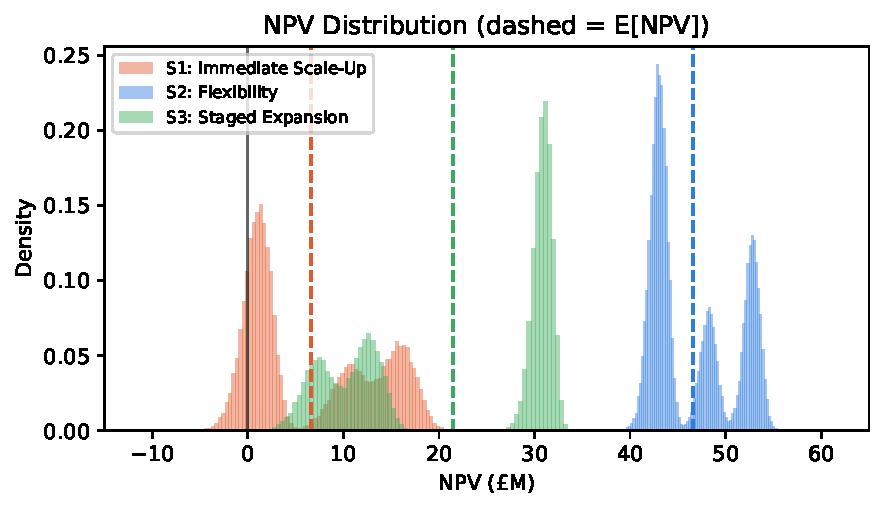
\includegraphics[width=0.5\linewidth]{fig_npv_dist.pdf}
    \caption{Simulated NPV density for each strategy (dashed lines = E[NPV]). S2 is tightly concentrated above \pounds40M; S1 has significant left-tail mass below zero.}
    \label{fig:npv_dist}
\end{figure}

%========================================================================================
\section{Recommendations}
%========================================================================================

\subsection{Strategic Recommendation: Adopt Strategy 2}

\textbf{GreenCo should adopt Strategy 2 (Flexibility and Risk Mitigation).} This recommendation is robust across all metrics: E[NPV] = \pounds46.5M (vs \pounds6.6M for S1 and \pounds21.6M for S3), zero probability of net loss, lowest NPV volatility, and highest VaR/CVaR. S2 dominates in every scenario (Table~\ref{tab:npv}), with no crossover point.

The fundamental reason is economic: the newsvendor cost structure (overage cost \pounds2800/t \textit{four times} the underage cost \pounds700/t) means GreenCo should produce conservatively and rely on spot markets for shortfalls. Adding large electrolyser capacity (S1/S3) exacerbates the overcapacity problem under low growth while providing only marginal benefit under high growth. Strategy 2 instead \textit{reduces demand uncertainty}, which simultaneously reduces both spot procurement waste (lower ELS) and inventory waste (lower ELOI)---addressing the root cause of profit variability rather than throwing capacity at it.

Under high growth, S2's systematic reliance on spot procurement from Year 3 is a genuine limitation. However, even in this scenario S2 yields NPV = \pounds52.75M (no comp.) or \pounds48.15M (with comp.), both far exceeding S1 and S3. If high growth materialises and spot market prices rise significantly, S2's pre-negotiated contingent contracts at \pounds2900/t provide important downside protection.

\subsection{Operational Recommendations}

\begin{enumerate}
    \item \textbf{Production policy:} Implement the newsvendor-optimal schedule $Q_t^* = \min(\mu_t + z^*\sigma_t,\,\bar{Q})$, reviewed annually as demand parameters update. Under Strategy 2, use $z^{*,S2} = \Phi^{-1}(0.125) = -1.150$ (reduced $c_s$ lowers the underage penalty, justifying further underproduction). \textit{Avoid planning at mean demand}---this ignores the asymmetric cost structure and the flaw of averages.

    \item \textbf{Refuelling station: add bays immediately.} The current M/M/3 configuration violates the 5-minute SLA at baseline ($W_q = 5.33$ min) and deteriorates rapidly under demand growth. \textit{This is independent of the investment strategy chosen.} Two additional bays ($s = 5$) are required for compliance across the 4-year horizon. With $s = 5$: $W_q = 0.24$ min at baseline, rising to 1.27 min under high growth by Y4. A single additional bay ($s = 4$) is insufficient under high growth (fails by Y4 at $\lambda = 14.64$/hr $> \lambda^{\max}_{s=4} = 14.44$/hr). The cost of non-compliance (contract breach) likely far exceeds the incremental bay installation cost.

    \item \textbf{Demand monitoring:} Under Strategy 2, the firm should monitor realised demand growth closely. If high growth materialises earlier than expected, activating an option to expand capacity (analogous to S3) at a premium cost may become worthwhile from Year 2 onward.
\end{enumerate}

\subsection{Limitations and Caveats}

\begin{itemize}
    \item \textbf{Demand independence:} Monthly demands are assumed i.i.d.\ within each year. Serial correlation (e.g.\ contract ramp-ups) would alter the newsvendor solution and widen the simulated NPV distribution.
    \item \textbf{Risk neutrality:} The analysis maximises E[NPV]. A risk-averse decision-maker would assign additional weight to downside outcomes; this would strengthen the case for S2 (already has zero loss probability) and weaken S1 further.
    \item \textbf{Flaw of averages:} Computing profits at expected demand $\mu_t$ rather than simulating monthly realisations underestimates costs due to the nonlinear capacity-demand interaction (Jensen's inequality). The Monte Carlo simulation explicitly addresses this; the analytical E[NPV] figures are close to but slightly above the simulated means (e.g.\ S2: \pounds46.52M analytical vs \pounds46.54M simulated).
    \item \textbf{Strategy 2 spot exposure under high growth:} From Year 3 onward under high growth, Strategy 2 relies systematically on spot procurement. If spot market liquidity is limited or prices spike, the pre-negotiated contingent contracts at \pounds2900/t are critical. If these contracts cannot be honoured at scale, S2's advantage would narrow.
    \item \textbf{Normal demand assumption:} Negative demand realisations are theoretically possible but negligible in practice ($>6\sigma$ from mean). Demand is truncated at zero in simulation.
    \item \textbf{Queueing model assumptions:} Steady-state M/M/$s$ assumes stationary Poisson arrivals. In practice, HGV arrivals may exhibit time-of-day patterns; a time-varying $\lambda(t)$ model would give a more accurate picture of peak congestion.
\end{itemize}

%========================================================================================
\begin{thebibliography}{9}
    \bibitem{gungor2026}
    E.~Gungor, \textit{3E3 Modelling Risk: Lecture Notes}, University of Cambridge, Lent 2026.
\end{thebibliography}

\end{document}
